%template1.tex
%The following LaTeX source file represents the simplest kind of slide presentation; no overlays, no included graphics. Substitute your favorite style for ``pascal''. To create the PDF file template1.pdf, (1) be sure to use the prosper class, then (2) execute the command latex template1.tex, and (3) the command dvipdf template1.dvi.

%%%%%%%%%%%%%%%%%%%%%%%%%%%%%%% template1.tex %%%%%%%%%%%%%%%%%%%%%%%%%%%%%%%%%%%
\documentclass[a4paper,blends,pdf,colorBG,slideColor]{prosper}
% definitions for slides for CSC544
% Lutz Hamel, (c) 2007

\hypersetup{pdfpagemode=FullScreen}

\usepackage{amssymb}
\usepackage{latexsym}
\usepackage{amsmath}
%\usepackage[usenames]{color}
\usepackage{xypic}


\newcommand{\term}[1]{\ensuremath{\mbox{\bf #1}}}
\newcommand{\nonterm}[1]{\ensuremath{\mbox{#1}}}
\newcommand{\ifstmt}[3]{\ensuremath{{\bf if}\; {#1}\;{\bf then}\;{#2}\;{\bf else}\;{#3}\;\term{end}}}
\newcommand{\whilestmt}[2]{\ensuremath{{\bf while}\; {#1}\;{\bf do}\;{#2}\; \term{end}}}
\newcommand{\funcstmt}[3]{\ensuremath{{\bf fun}\; {#1}\; {\bf is}\; {#2} \; {\bf return}\; {#3}}}
\newcommand{\syntaxset}[1]{\ensuremath{\mbox{\bf #1}}}
\newcommand{\orbar}{\;|\;}
\newcommand{\bs}[1]{\begin{slide}{#1}\ptsize{8}}
\newcommand{\es}{\end{slide}}
\newcommand{\co}{\,\colon\;}
\newcommand{\pair}[2]{\ensuremath{\langle {#1}, {#2} \rangle}}
\newcommand{\encode}[1]{\ensuremath{\langle {#1} \rangle}}
\newcommand{\mytab}{\makebox[.15in]{}}
%\newcommand{\abs}[1]{{\mid{#1}\mid}}
\newcommand{\abs}[1]{{|{#1}|}}
\newcommand{\ol}[1]{\overline{#1}}

\newcommand{\qaccept}{\ensuremath{q_{\mbox{\tiny accept}}}}
\newcommand{\qreject}{\ensuremath{q_{\mbox{\tiny reject}}}}
\newcommand{\accept}{{\em accept}}
\newcommand{\reject}{{\em reject}}

\newcommand{\machine}[1]{
	\begin{quote}
	{#1}
	\end{quote}
	}

\newcommand{\fdef}[1]{
	\begin{center}
	\fbox{
	\begin{minipage}{3.5in}
	{\bf Definition:}
	{#1}
	\end{minipage}
	}
	\end{center}
	}

\newcommand{\ftheorem}[1]{
	\begin{center}
	\fbox{
	\begin{minipage}{3.5in}
	{\bf Theorem:}
	{#1}
	\end{minipage}
	}
	\end{center}
	}

\newcommand{\flemma}[1]{
	\begin{center}
	\fbox{
	\begin{minipage}{3.5in}
	{\bf Lemma:}
	{#1}
	\end{minipage}
	}
	\end{center}
	}


\newcommand{\fframe}[1]{
	\begin{center}
	\fbox{
	\begin{minipage}{3.5in}
	{#1}
	\end{minipage}
	}
	\end{center}
	}

\newcommand{\nframe}[1]{
	\begin{center}
	\begin{minipage}{3.5in}
	{#1}
	\end{minipage}
	\end{center}
	}

\begin{document}

\bs{Parallel Computation}

Parallel computation is the use of machines that allow for the execution of
multiple computation steps simultaneously.

We have encountered some form of parallelism already in the form of nondeterministic Turing machines.  However, this parallelism is limited since there is no communication allowed between the computational branches.

Here we investigate a model of parallelism that is more realistic: deterministic processing elements and communication between the elements.

Since our processing elements are deterministic we will see that class of decision problems amenable to parallelization is (most likely) a subset of $P$.
\es

\bs{Matrix Multiplication}
{
We start our investigation by examining a problem that can be readily executed in parallel: matrix multiplication.

Given two $m\times m$ matrices $A$ and $B$, the product $C = A \times B$ is
defined as
\[
c_{ij} = \sum_{k = 1}^m a_{ik} \times b_{kj}, \mbox{ for $i,j = 1,\ldots,m$}.
\]
Let $n = 2m^2$, then it is easy to see that a straightforward sequential implementation of this algorithm will execute in $O(m^3) = O((\sqrt{\frac{n}{2}})^3) = O(n^{3/2})$ time.

The question is, if we had just the right parallel machine, what would be the execution time then?
}
\es

\bs{Parallel Matrix Multiplication}
{\small  Assume that we had just the right number of processors, then we could embed
the computation on the parallel machine as follows, assuming a $3\times 3$ multiplication problem:

\begin{center}
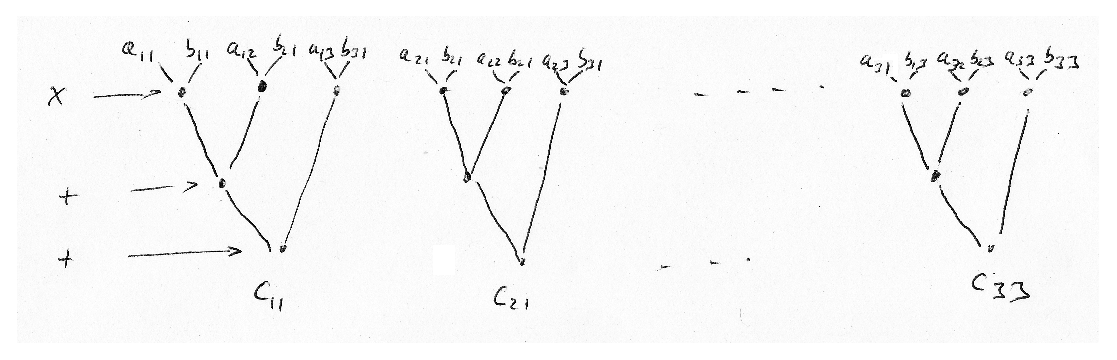
\includegraphics[height=30mm]{images/pmult.eps}
\end{center}

Note that we assume $(3 + 2)m^2=m^3+2m^2$ processors (with $m = 3$ for our example).  
In other words, we assume $O(m^3) = O(n^{3/2})$ processors.  Observe that our
total execution time characterized by the depth of the layers of processors
drops to $O(\log m) = O(\log n^{3/2})=O(\frac{1}{2}(\log n - \log 2)) = O(\log n)$.

This means, given just the right machine we can go from polynomial time to logarithmic time.
}
\es

\bs{Circuits}
{\small
The idea of `just the right machine' gives us a way to characterize parallizability of problems.

We do this via the notion of {\bf\em circuits}.  Circuits are constructed from gates and we view each gate as an extremely simple processor.  By connecting these processors we obtain a {\bf\em parallel machine} since each of the processors can perform work independently as soon as input is available. Formally,

\fdef{A {\bf\em Boolean circuit} is a collection of {\bf\em gates} and {\bf\em inputs}
connected by {\bf\em wires}.  Cycles are not permitted.  Gates can take three forms:
$AND$, $OR$, and $NOT$ gates.}
\begin{center}
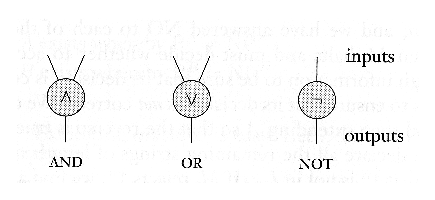
\includegraphics[height=20mm]{images/circuit-elements.eps}
\end{center}

\begin{center}
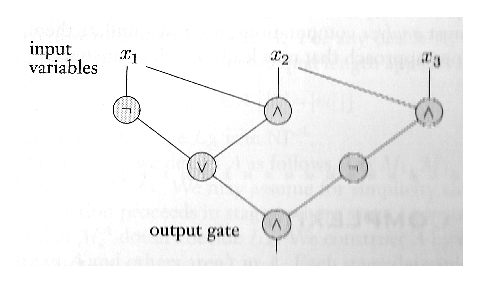
\includegraphics[height=20mm]{images/circuit.eps}
\end{center}

}
\es

\bs{Circuit Matrix Multiply}
{\small
Given two binary $m\times m$ matrices $A$ and $B$, the binary product $C = A \wedge B$ is
defined as
\[
c_{ij} = \bigvee_{k = 1}^m a_{ik} \wedge b_{kj}, \mbox{ for $i,j = 1,\ldots,m$}.
\]
Our $3\times 3$ example is then,
\begin{center}
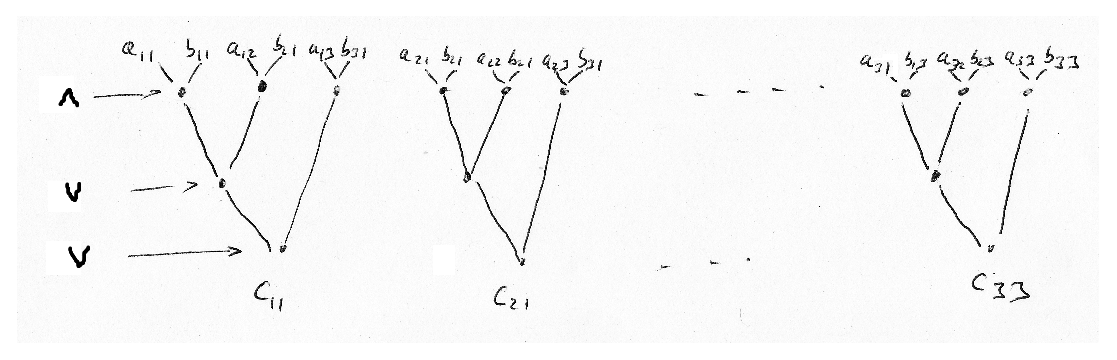
\includegraphics[height=30mm]{images/pmult-bin.eps}
\end{center}
Note, all the prior analysis still holds, the only difference is that we now have only very simple processors.
}
\es

\bs{Circuit Families}
{\small
Note, in general we can use circuits as deciders: \[f_C\co \{0,1\}^n \rightarrow \{0,1\}.\]
That is, given a string $w \in \{0,1\}^n$, the circuit implementing the function $f_C$
can answer the question $w \stackrel{?}{\in} L(C)$.

This means we can use circuits as general representations of algorithms (Perhaps not surprising since computers are made up of circuits).

One of our assumption was that we have always the exact circuit available for our problem, or in other words, there is always a circuit available whose $n$ matches the string we want to decide.

\fdef{A {\bf\em circuit family} $C$ is an infinite list of circuits  $(C_0, C_1, \ldots)$,
where $C_n$ has $n$ input variables.  We say that $C$ decides a  language
$A$ over $\{0,1\}$ if, for every string $w$,
\[
w \in A \mbox{ iff } C_n(w) = 1,
\]
where $\abs{w} = n$.
}
}
\es

\bs{Parallel Complexity}

\fdef{We define the {\bf\em parallel processor complexity} of a Boolean circuit to be its {\em size}.  We define the {\bf\em parallel time complexity} of a Boolean circuit to be its {\em depth}, or the longest distance from an input variable to an output gate.}

The complexity of a parallel algorithm is always given as a pair \[\encode{\mbox{\em processor complexity}, \mbox{\em time complexity}}.\]

For our Boolean matrix multiplication example we have a parallel complexity of 
\[\encode{O(n^{3/2}), O(\log n)}.\]
\es


\bs{The Class $L$}

The class $L$ is the class of languages that is decidable in $log(n)$-space,
\[
L = \{ A | \mbox{$A$ is decidable a in $log(n)$-space deterministic TM}\}
\]

Observation: $ L \subseteq P$
\es

\bs{The Class $NC$}
Before we can define the class of all parallel algorithms we need one more technical definition,
\fdef{A family of circuits $C_k$, $k = 1, 2, \ldots$, is {\bf\em uniform} if some log space transducer $T$ outputs $\encode{C_n}$ when $T$'s input is $1^n$.
}

This definition says that given a specification of a circuit, the circuit can be constructed easily. 

This avoids the problem that we can assume that we can construct circuits that solve the $TSP$ problem easily.

\fdef{For $i \ge 1$ let $NC^i$ be the class of languages that can be decided by a uniform family of circuits with polynomial size and $O(\log^i n)$ depth. Let
\[
NC = \bigcup_i NC^i, \mbox{ for $i \ge 1$}.
\]
}

\es

\bs{The Class $NC$}
{\small
\ftheorem{
\[
NC \subseteq P
\]}
{\bf Proof:} A polynomial time algorithm can run the log space transducer to generate circuit $C_n$ and then simulate it on an input of length $n$. $\Box$

Now, is $NC = P$?  Probably not, since $P$ contains a number of inherently sequential problems.
}
\es

\bs{Finally!}
Observation: $L \subseteq NC \subseteq P \subseteq NP \subseteq PSPACE \subseteq EXPTIME$
\es

\bs{Overview}
\begin{center}
    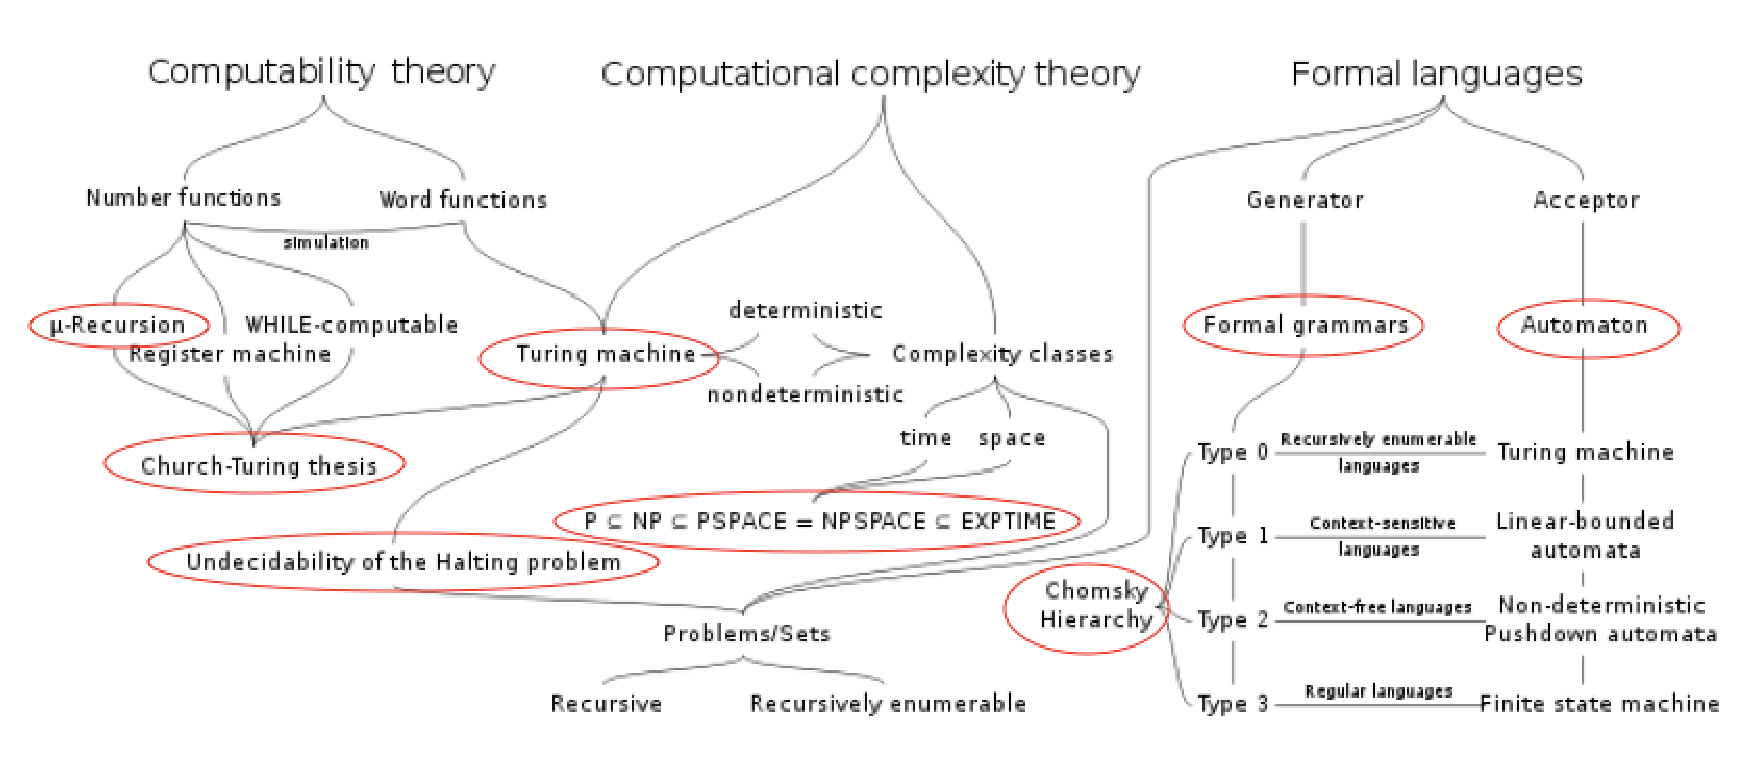
\includegraphics[height=45mm]{images/course-road-map-00.eps}
\end{center}

\es

\end{document}
%%%%%%%%%%%%%%%%%%%%%%%%%%% end of template1.tex %%%%%%%%%%%%%%%%%%%%%%%%%%%%%%%%

